\section{move base}

The move base package is the most important part of the ROS navigation stack and is used for path planning, both local planning and global planning. Therefore the move base package takes a goal pose as input and calculates the velocity commands necessary for the robot to reach the goal. Figure \ref{move_base} gives an overview the package components. 

\begin{figure}[h]
  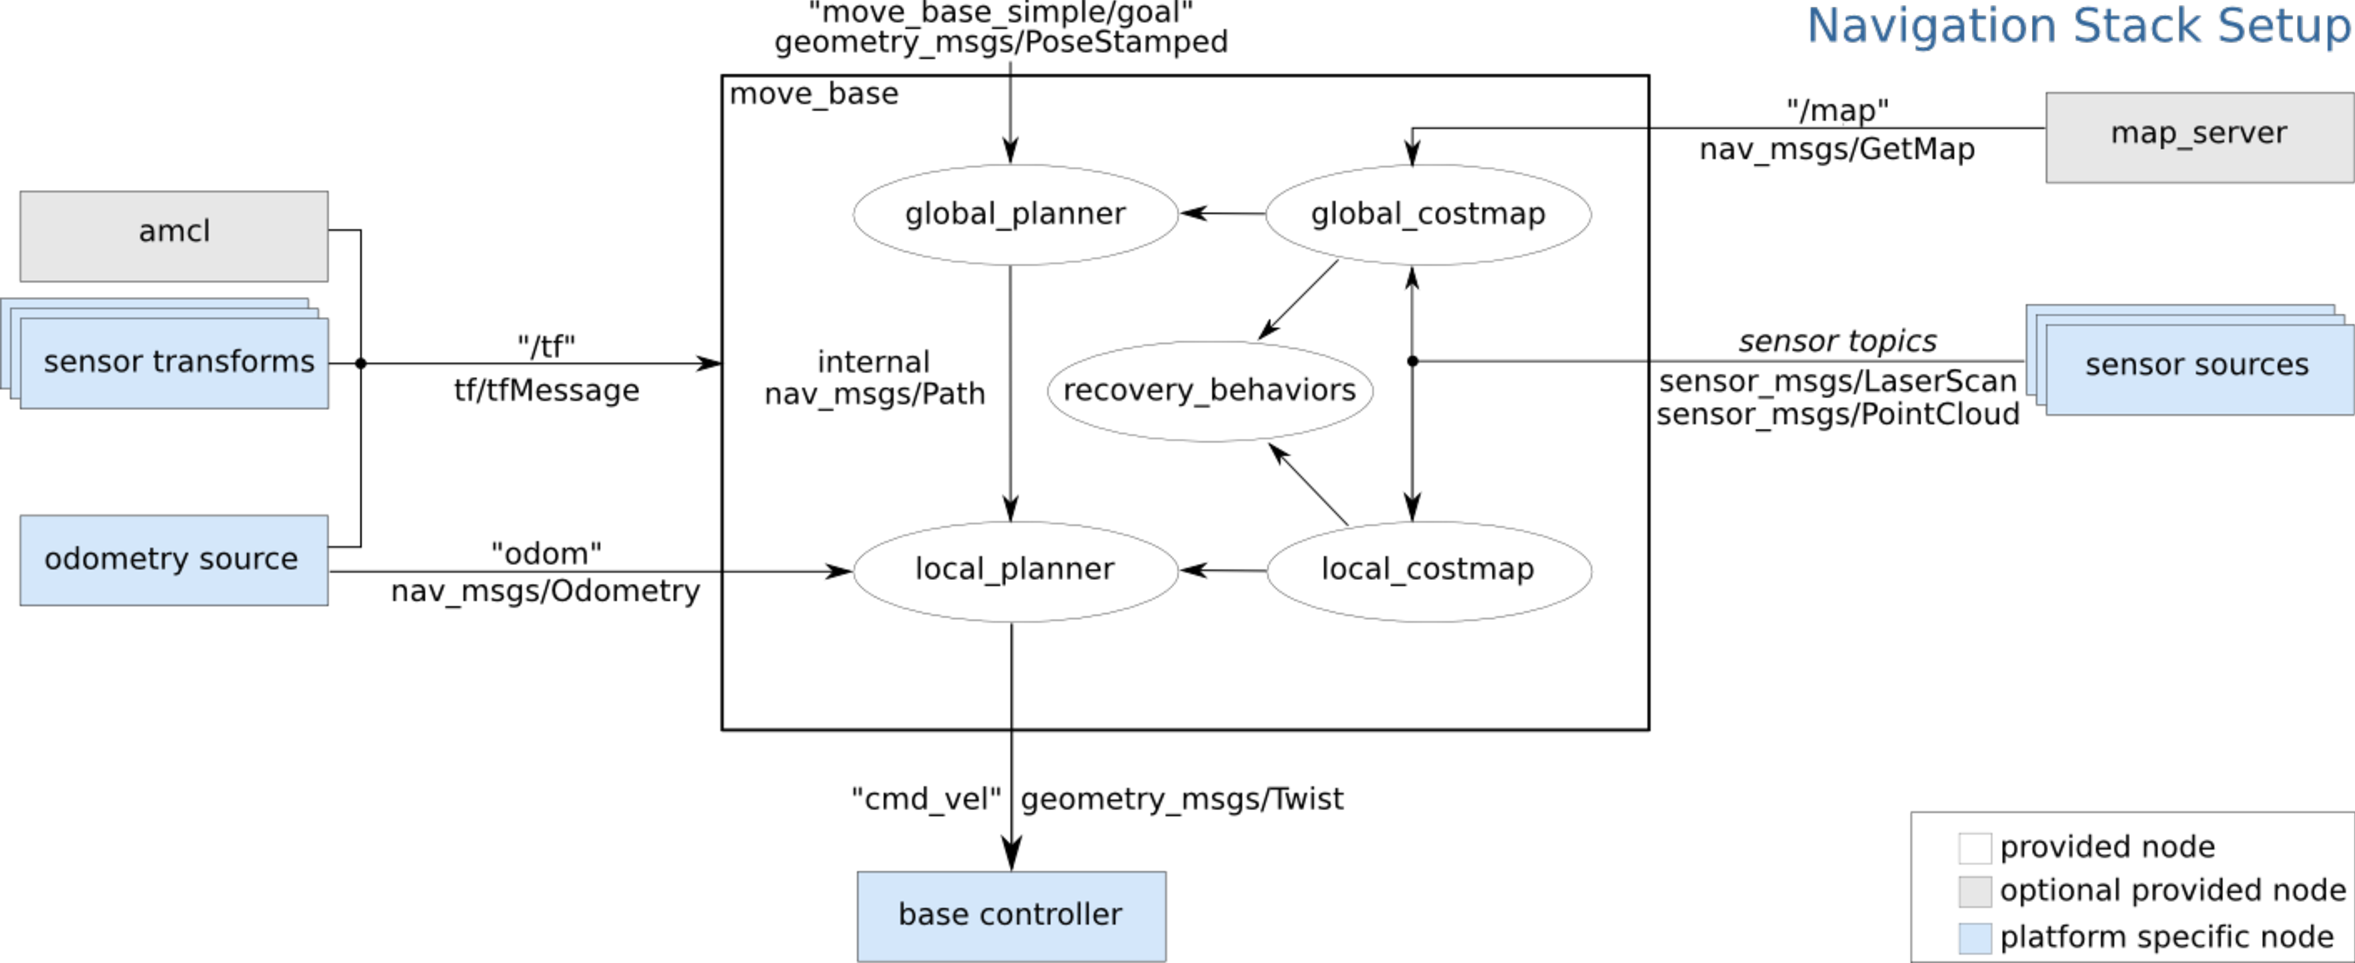
\includegraphics[width=1.02\textwidth]{figures/move_base.pdf}
  \caption{move base structure}
  \label{move_base}
\end{figure}

The split of the package into components is useful as each component can be chosen seperately to fit to the robot. There are two costmap components, one for the local planner and one for the global planner. Costmaps are grid maps with each cell containing information about how much the planner should avoid the cell. The cost is very high around obstacles and decreasing with increasing distance to obstacles. The global costmap is usually built based on a global map, which has to be provided. The local costmap on the other hand is used in the local planner and contains information about obstacles in the near surrounding of the robot. It is build using the information of laser scanners or other sensors used for obstacle detection. The global planner creates a path from the current location to the goal based on the global costmap. Based on the global plan and the local costmap the local planner then calculates the actual velocities sent to the base controller. The recovery behaviors component is used to unstuck the robot in case no valid global or local plan is found.